
\documentclass[aspectratio=169]{beamer}
\usetheme{metropolis}           % Use metropolis theme
\usepackage[utf8]{inputenc}
\usepackage{graphicx}
\usepackage{eso-pic}
\usepackage{graphics}
\usepackage{tikz}
\usepackage[export]{adjustbox}
\usepackage{multicol}
\usepackage{listings}
\usepackage{helvet}
\usepackage{booktabs}
\usepackage{threeparttable}
\usepackage{fontspec}


\title{Stata Track 1 - Topic 2 \newline Data Management and Cleaning}
\date{\today}
\author{Meyhar Mohammed, Kristoffer Bjarkefur} % Name of author(s) of session here
\institute{Development Impact Evaluation (DIME) \newline The World Bank }
\setbeamercolor{background canvas}{bg=white}	% Sets background color

% The below command places the World Bank logo and DIME logo to the right corner
\titlegraphic{%
	\begin{picture}(0,0)
	\put(330,-180){\makebox(0,0)[rt]{
\includegraphics[width=3cm]{../../img/WB_logo}}}
	\end{picture}%
	\begin{picture}(0,0)
	\put(390,-180){\makebox(0,0)[rt]{
\includegraphics[width=1.5cm]{../../img/i2i}}}
	\end{picture}%
}

%%% Section page with picture of Light bulb
\makeatletter
\defbeamertemplate*{section page}{mytheme}[1][]{
	\centering
	\begin{minipage}{22em}
		\raggedright
		\usebeamercolor[fg]{section title}
		\usebeamerfont{section title}
		\par
		\ifx\insertsubsectionhead\@empty\else%
		\usebeamercolor[fg]{subsection title}%
		\usebeamerfont{subsection title}%
		\fi
		\ifstrempty{#1}{}{%
			\includegraphics[width=100mm, height=60mm]{#1}%
		}
		\insertsectionhead\\[-1ex]
		\insertsubsectionhead
		\usebeamertemplate*{progress bar in section page}

	\end{minipage}
	\par
	\vspace{\baselineskip}
}
\makeatother

%%% Define a command to include picture in section,
%%% make section, and revert to old template
\newcommand{\sectionpic}[2]{
	\setbeamertemplate{section page}[mytheme][#2]
	\section{#1}
	\setbeamertemplate{section page}[mytheme]
}

\usepackage{fancyvrb} % Allows customization of verbatim environments
%Fancyvrb docs: http://mirrors.ibiblio.org/CTAN/macros/latex/contrib/fancyvrb/doc/fancyvrb-doc.pdf
\fvset{fontsize=\scriptsize} % The font size of all verbatim text can be changed here

%So we can use option FloatBarrier, which is similar to [H] but is an
%alternative solition when the algorithm can't solce [H] as too many
%settings are going on. [H] seems to get stuck in infinite loop
%https://tex.stackexchange.com/questions/2275/keeping-tables-figures-close-to-where-they-are-mentioned
\usepackage{placeins}
\newcommand{\codeexample}[2]{
	\begin{figure}
		\VerbatimInput[
		framesep=3mm,
		frame=lines, % line above and below code section
		numbers=left, %Line number
		label= #1, %name of code section
		baselinestretch=0.90, %Use line space more similat to line space in code editors
		]{#2} %Write the relative file path and the name of the file to be included
	\end{figure}
	\FloatBarrier
}


%% The below command creates the ligh bulb logos in the top right corner of the
\begin{document}

{
	\usebackgroundtemplate{
\includegraphics[height=55mm, right]{../../img/top_right_corner.pdf}}
	\maketitle
}

%%%%%%%%%%%%%%%%%%%%%%%%%%%%%%%%%%%%%%%%%%% heading of section 1
\sectionpic{Think reproducible}{../../img/section_slide}


\begin{frame}{Outline}
	\begin{enumerate}
		\item Folder organization
		\item Master do-files
		\item First overview of a data set
		\item Master data sets
		\item Basic data cleaning tasks:
			\begin{itemize}
				\item Unique ID
				\item Variable and value labels
				\item Missing values
				\item Check for outliers
			\end{itemize}
	\end{enumerate}
\end{frame}


\begin{frame}{Data Management}
	\begin{itemize}
		\item The first part of this presentation will introduce you to some data management practices
		\item We have one standard almost all projects are following. You do not have to follow exactly our model, but you MUST have one model and organize your project accordingly, otherwise you will make mistakes in your data
		\item We have tools and manuals for how to set up our model, but they are out of the scope of this training, but we will explain what any model should include by using our model as an example
	\end{itemize}
\end{frame}

\begin{frame}{Folder Organization
- Sample Folder Structure}
	\begin{figure}
		\centering
		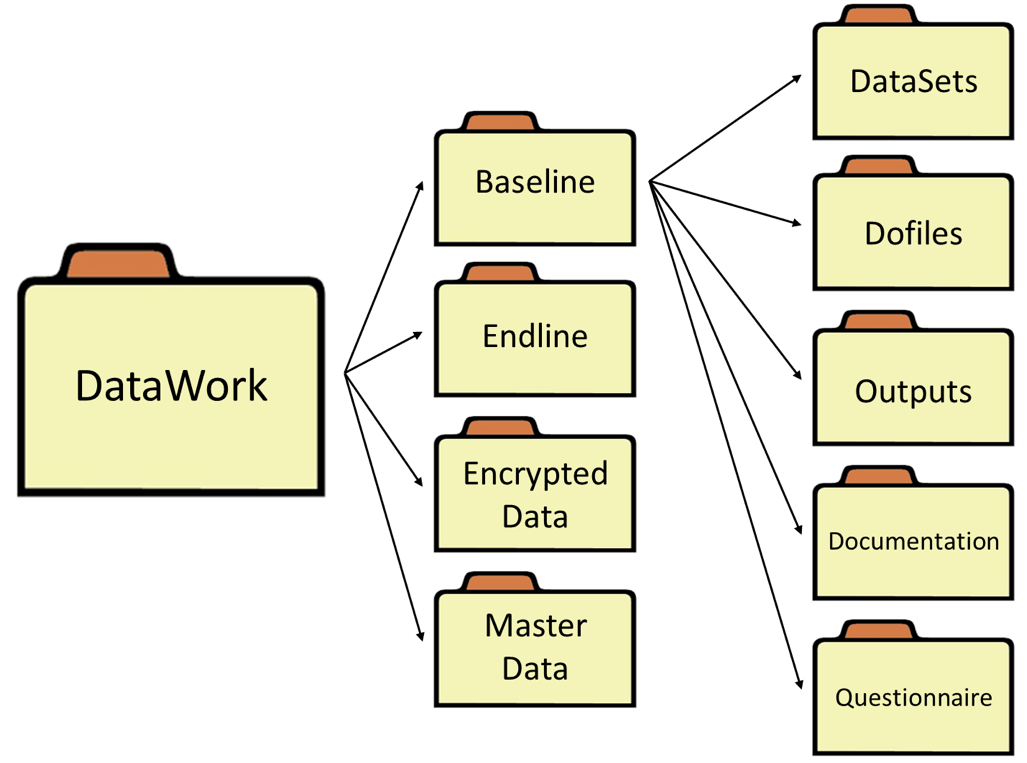
\includegraphics[width=.7\linewidth]{img/folderstructure}
	\end{figure}
\end{frame}

\begin{frame}[fragile]{Where to put data?}
	\begin{columns}[c]
		\column{.45\linewidth}
		\begin{itemize}
			\item Raw data with identifying information should be stored in the EncryptedData folder
			\item All data in the Intermediate or the Final folder should be de-identified
			\item Use VeraCrypt to encrypt the EncryptedData folder
		\end{itemize}

		\column{.55\linewidth}
		\begin{figure}
			\centering
			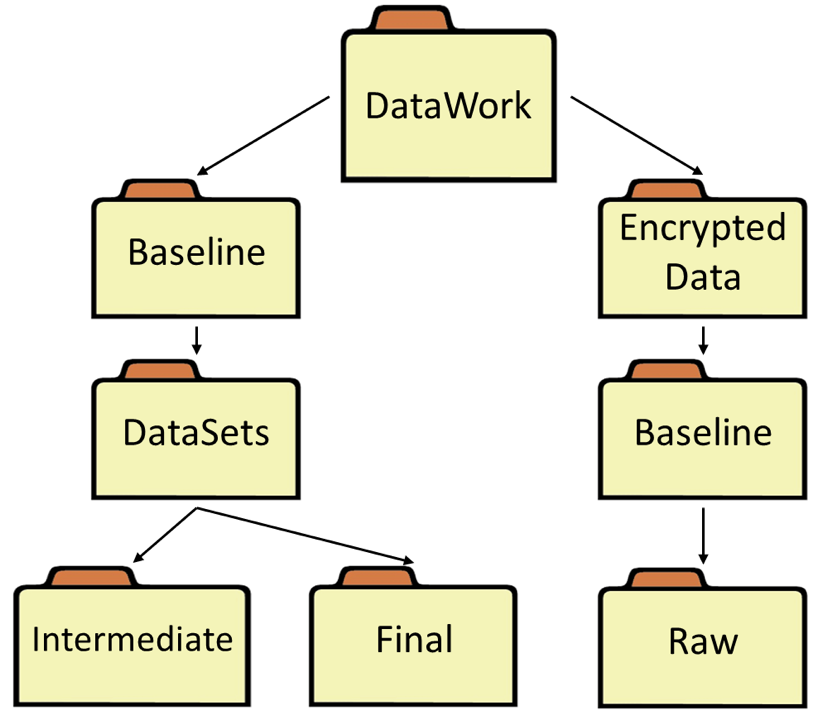
\includegraphics[width=\linewidth]{img/folderstructure2}
		\end{figure}
	\end{columns}
\end{frame}

\begin{frame}{What is a Master do-file?}
	\begin{itemize}
		\item You can make a do-file run other do-files. This is the most important thing a master do-file does.
			\begin{itemize}
				\item First, run do-file 1
				\item Then, run do-file 2
				\item Then, run do-file 3, etc.
			\end{itemize}
		\item Using master do-files as a map to the DataWork folder, the person writing the do-files can tell a person trying to understand the do-files which order to read and run them
		\item Without a master do-file, you either need one extremely long do-file, or write instructions in which order to run all the do-files
	\end{itemize}
\end{frame}

\begin{frame}{Exempt from a Master do-file}
	This do-file first run the do-file \texttt{cleaning.do} and then the \texttt{analysis.do}
		\codeexample{run-do-from-do.do}{code/run-do-from-do.do}
	This tells both, Stata and humans reading the code in which order the do-files should be run
\end{frame}

\begin{frame}[fragile]{Master do-file : Allows easy collaboration}
\codeexample{master-dofile-rootpath.do}{code/master-dofile-rootpath.do}
\end{frame}

\begin{frame}{Master do-file - The map to all data work}
	\begin{itemize}
		\item At the end of every round of a project:
		\begin{itemize}
			\item 	You should be able to reproduce all your work from raw data to all outputs with one click in this do-file
			\item Anyone should be able to follow and to reproduce all your work form raw data to all outputs with one click in this do-file, after adding only their root folder path
		\end{itemize}
	\end{itemize}
\end{frame}

\begin{frame}[fragile]{Master do-file - Allows easy collaboration}
	\begin{itemize}
		\item If we share a project over DropBox or OneDrive all team member have the same folder structure
		\item A master do-file allows multiple people to set their own global to the project folder
		\item This way anyone sharing the project folder can easily run your do-files
	\end{itemize}
\end{frame}

\begin{frame}{Task 1 - Set up the Master do file}
	\begin{itemize}
		\item See the folder called \texttt{ST1} that we have provided. It is a simplified example of our folder structure the way our command \texttt{iefolder} sets up. How to use \texttt{iefolder} and all features of our folder structure set up is out of the scope for this session. That is why we provide a simplified version
		\item Copy this folder to somewhere on the computer you are using. All the work we will do from now, will be in this folder 
		\item Find the do-file \texttt{ST1\_MasterDofile.do} file in this folder and open it, find the root-path section shown below and update it with your root-path
	\end{itemize}

\codeexample{master-dofile-rootpath-short.do}{code/master-dofile-rootpath-short.do}
\end{frame}

\begin{frame}{Task 1 - Set up the Master do file}
	\begin{itemize}
		\item Keep working in \texttt{ST1\_MasterDofile.do}. Find the section below. After \texttt{\$\string{ST1\_do/\string}} enter the name of the do-file you write for topic 1 in the previous session
		\item Now you must move the do-file from topic 1 to the location that \texttt{\$\string{ST1\_do/\string}} is pointing to. To find what that location is, you must follow the globals defined above this section.
		\item When you have moved the do-file, change the local \texttt{topic1} to 1 and run your do-file. What happened? Did you also run your do-file from topic 1?
	\end{itemize}
	
	\codeexample{master-dofile-rundo.do}{code/master-dofile-rundo.do}
\end{frame}


\begin{frame}{Task 2 - Update the topic 1 do-file}
	\begin{itemize}
		\item Move the data set \texttt{endline\_data\_raw\_nodup.dta} to the \texttt{ST1/DataSets/Deidentified} folder
		\item In your do-file for topic 1, where you have \newline \texttt{use "\$\string{folder\_Lab1\string}/Data/endline\_data\_raw\_nodup.dta", clear} replace the global to use the \texttt{\$\string{ST1\_dtDeID\string}} global created in your master do-file, and remove the \texttt{Data/} part of the path, i.e. \newline  \texttt{use "\$\string{ST1\_dtDeID\string}/endline\_data\_raw\_nodup.dta", clear}
		\item Similarly, replace the global in \newline \texttt{save "\$\string{folder\_Lab1\string}/Data/endline\_data\_post\_topic1.dta", replace} to the \texttt{\$\string{ST1\_dtInt\string}} global (note that it is not the same global as above), i.e. \newline  \texttt{save "\$\string{ST1\_dtInt\string}/endline\_data\_post\_topic1.dta", replace}
	\end{itemize}

\end{frame}

\begin{frame}{Keep using the folder you created}
	\begin{itemize}
		\item Through the rest of this training we recommend that you can create a do-file for each topic, and add them all to the master do-file. Soon our tasks will depend on edits you made to your data set in a previous topic, and then it is great that you can replicate your data sets
		\item This is similar to how we want you to run a DIME project. More on how this is set up in an actual project in track 2, but the principles are the same as shown here
		\item A do-file is instructions for a task, and this system of folders and master do-files is how these task instructions becomes instructions for a full project
	\end{itemize}
\end{frame}

%%%%%%%%%%%%%%%%%%%%%%%%%%%%%%%%%%%%%%%%%%%%%%%%%%%55
\sectionpic{Explore a new data set}{../../img/section_slide}

\begin{frame}{Explore a new data set}
	\begin{itemize}
		\item We have already seen some practical commands to explore a data set (\texttt{describe}, \texttt{tabulate} etc.), but this section introduce you to some theoretical concepts equally important when exploring a data set for the first time
		\item What is the first thing you want to look for every single time you open a new data set for the first time?
		\begin{itemize}
			\item Unit of observation
			\item Uniquely and fully identifying ID variable
		\end{itemize}
	\end{itemize}
\end{frame}



\begin{frame}{Explore a raw data set}
	\begin{itemize}
		\item \texttt{Household\_data.csv}
		\begin{figure}
			\centering
			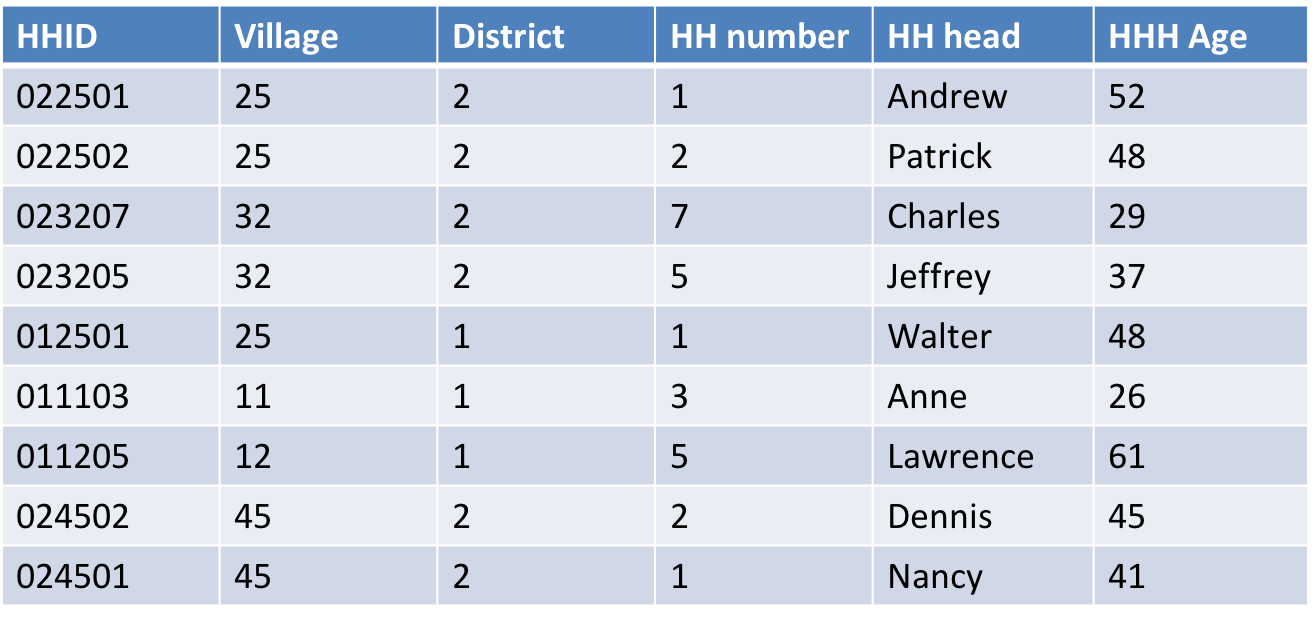
\includegraphics[width=\linewidth]{img/raw1}
		\end{figure}
	\end{itemize}
\end{frame}



\begin{frame}{Explore a raw data set}
	\begin{itemize}
		\item \texttt{Clinic\_data.csv}
		\begin{figure}
			\centering
			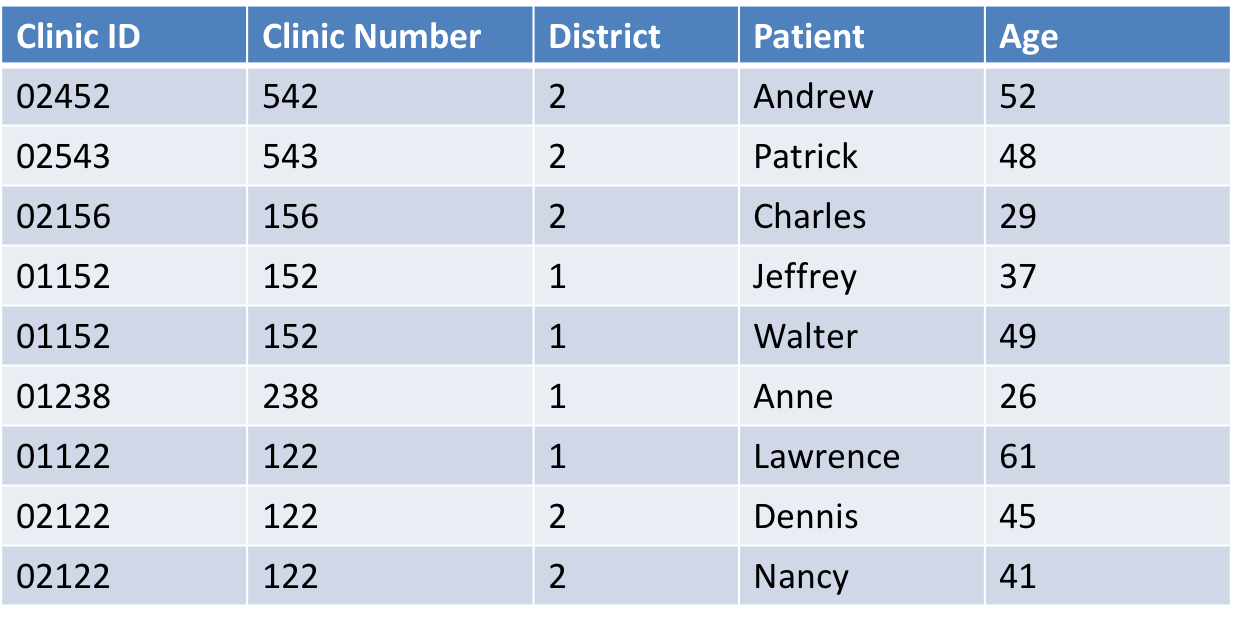
\includegraphics[width=\linewidth]{img/raw2}
		\end{figure}
	\end{itemize}
\end{frame}


\begin{frame}{First thing to check}
	\begin{itemize}
		\item Unit of observation check list when opening a new data set:
		\begin{itemize}
			\item What does each row represent?
			\item Which variable do you think is the main ID uniquely identifying each row?
			\item Test that the variable indeed is uniquely and fully identifying
			\begin{itemize}
				\item Stata commands: \texttt{isid} and \texttt{codebook}
			\end{itemize}
		\end{itemize}
	\end{itemize}
\end{frame}


\begin{frame}{Task 3 - Test of unit of observation}
	\begin{itemize}
		\item Re-run \texttt{ST1\_MasterDofile.do} that you edited in the last task. Make sure that after it runs you are still in the \texttt{endline\_data\_raw\_nodup.dta} data set.
		\begin{itemize}
			\item What is the unit of observation, i.e. what does each row represents?
			\item Which variable do you think is the variable that uniquely and fully identifies the data set?
			\item Test the variable to make sure that is the unique ID variable
		\end{itemize}
		\item Create a new do-file for this session. Save it in the same folder as the do-file from topic 1, and then make sure that the new do-file also runs from the master do-file. 
		\item Then in that do-file, open the data using \newline \texttt{use "\$\string{ST1\_dtInt\string}/endline\_data\_post\_topic1.dta", clear}
		\item Then add to the new do-file the tests you do to verify which variable is the ID variable in the data set.
	\end{itemize}
\end{frame}

%%%%%%%%%%%%%%%%%%%%%%%%%%%%%%%%%%%%%%%%%%%%%%%%%%%
\sectionpic{Master Data Sets}{../../img/section_slide}


\begin{frame}{What is a Master data set?}
	\begin{itemize}
		\item With multiple data set you need to have a tool to keep track of your observations across different data collections and over time. You guessed it – that tool is master data sets!
		\item A master data set should include all observations the project has ever encountered. Not just observations assigned to treatment or sampled for data collection
		\item A master data set should include information relevant across data set that is constant across the project
		\begin{itemize}
			\item Uniquely identifying ID
			\item Treatment assignment
			\item Sampling
			\item Monitoring status
		\end{itemize}
	\end{itemize}
\end{frame}


\begin{frame}[fragile]{Data Management -
Master Data}
	\begin{columns}[c]

		\column{.45\linewidth}
		\begin{itemize}
			\item For each unit of observation you have one encrypted master data set, and one available to all
			\item The encrypted data set has unique ID and identifying information
			\item The other one should not include any identifying information
		\end{itemize}

		\column{.55\linewidth}
		\begin{figure}
			\centering
			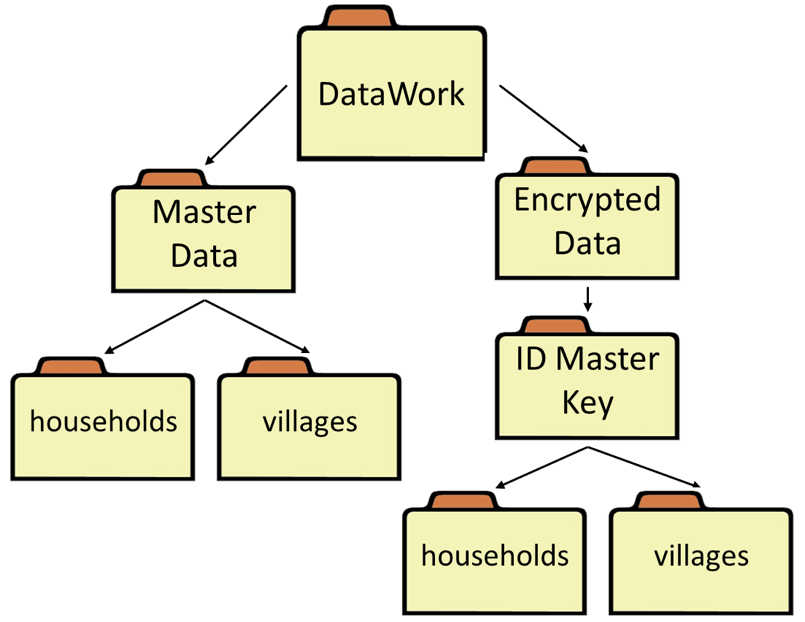
\includegraphics[width=\linewidth]{img/datamanage1}
		\end{figure}
	\end{columns}
\end{frame}

%%%%%%%%%%%%%%%%%%%%%%%%%%%%%%%%%%%%%%%%%%%%%%%%%%%
\sectionpic{Data Cleaning}{../../img/section_slide}


\begin{frame}{Role division in cleaning the data}
	\begin{itemize}
		\item Field Coordinator / Research Assistants
		\begin{itemize}
			\item No one will look at the data as much as the FC/RA
			\item Irregularities in the data that the FC/RA does not identify will often never be discovered
		\end{itemize}
		\item Principle Investigators
		\begin{itemize}
			\item In charge of deciding which irregularities will be corrected and how
			\item Never make any decision on data reformatting without talking to PIs
			\item PIs completely depend on FCs/RAs to identify irregularities and get the information to make the best call
			\item Of course, this all comes up when the PI starts writing up the analysis
			\item E.g. we sampled 4,567 HHs and we only have 3,897 in the regressions …
		\end{itemize}
	\end{itemize}
\end{frame}

\begin{frame}{Data Cleaning Tasks}
	\begin{center}
		\begin{tabular}{ p{6.5cm}|p{6.5cm} }			
			\multicolumn{1}{c}{\Large Format the data set} & \multicolumn{1}{c}{\Large Edit the dataset} \\
			\hline
			\textbullet Make the data easier to work with for yourself, your team and other researchers \newline
			\textbullet Document the knowledge you have about the data now. You will soon forget 
			& \textbullet Remove data points that will bias the analysis or make the analysis invalid in any other way  \\
			\hline
			1. Rename variables \newline 2. Remove strings \newline 3. Variable and value labels & 1. Standardize units \newline 2. Handle missing values \newline 3. Check for outliers  \\
			\hline  
		\end{tabular}	
	\end{center}
\end{frame}	
	
\begin{frame}{Naming conventions}
	\begin{itemize}
		\item Do not change the names of variables coming from a survey
		\item Keep all variables collected with survey data the same as in the questionnaire. Even if you do not like the naming conventions used in the questionnaire
		\item Exception: In a loop over, for example, crops where a variable like harvest is asked for each crop and automatically named, \texttt{harvest\_1}, \texttt{harvest\_2} etc., then those can be renamed to \texttt{harvest\_crop1}, \texttt{harvest\_crop2} etc., or \texttt{harvest\_c1}, \texttt{harvest\_c2} etc.
	\end{itemize}
\end{frame}

\begin{frame}{No string variables in the final data }
	\begin{itemize}
		\item Exceptions:
		\begin{itemize}
			\item Proper nouns that are not categories
			\item Digits with leading zeros or long IDs (over 15 digits)
		\end{itemize}
		\item Categorical string variables must be made numeric with value labels
		\begin{itemize}
			\item See \texttt{encode}
			\item Best practice using encode includes using both the \texttt{label()} and the \texttt{noextend} option
		\end{itemize}
	\end{itemize}
\end{frame}

\begin{frame}{Variable and value labels }
	\begin{itemize}
		\item We already introduced labels in the first lab. When cleaning a data set you should also make sure that all variables are properly labeled
		\item Check all variables have variable labels (in English or the language used in the research team)
		\item Check all that all categorical variables have value labels (in English or the language used in the research team)
		\item Useful commands: \texttt{label variable}, \texttt{label define}, \texttt{label value}, \texttt{label dir}, \texttt{label list}
	\end{itemize}
\end{frame}

\begin{frame}{Standardize units }
	\begin{itemize}
		\item Quantity variables should be converted into standardized units. One unit for weight (usually kg), length/distance (usually meter), etc.
		\item Often a difficult task due to usage of local non-standardized units. Use field team to collect as much information about local units and then decide on a conversion rate together with your PI
	\end{itemize}
\end{frame}


\begin{frame}{Missing values - Survey codes}
	\begin{itemize}
		\item During surveys missing answers are recorded using different codes. Like -88 for “I do not know” or -999 for “Declined to answer”
		\item We need to turn these survey codes to missing values since -88 or -999 will distort averages and other calculations
		\item Use any value of \texttt{.a}, \texttt{.b} etc. to represent “I do not know”, another one for “Declined to answer”, and another for each other missing answer code you have
		\item Be consistent across your data set. If you pick \texttt{.a} for “Do not know” then use \texttt{.a} to represent that in all variables in your data set
		\item Use the command summarize is efficient to find codes for missing answer as they stand out as negative values (that is why we use negative values as missing answer codes)
	\end{itemize}
\end{frame}



\begin{frame}{Outliers - identifying}
	\begin{itemize}
		\item We do not want our results to be driven by a few individuals. For example, the village leaders get all benefits
		\item No exact rule for what is an outlier.  Ask if your PI for preference of specific rule
		\item Identifying outliers often comes down to common sense
		\item Can the outlier be explained by typos? Especially common when selecting units from multiple choice lists
		\item Useful commands: \texttt{sum detail}, \texttt{tabulate}, \texttt{inspect}, \texttt{assert}, \texttt{histogram}
	\end{itemize}
\end{frame}


\begin{frame}{Outliers -
How to deal with outliers?}
	\begin{itemize}
		\item This is ultimately the decision of the researcher
		\item The goal is to deal with them while losing as little information as possible
		\begin{itemize}
			\item Delete observations
			\begin{itemize}
				\item Almost never desired as it loses a lot of information in variables that were correct
			\end{itemize}
			\item Delete specific data point (i.e. replace to missing)
			\begin{itemize}
				\item Frequently used but the observation would be dropped in regressions using that variable
			\end{itemize}
			\item Winsorization is a method were observations are not dropped, neither from the data set or from regressions
		\end{itemize}
	\end{itemize}
\end{frame}

\begin{frame}{Outliers - Winsorization}
	\begin{itemize}
		\item This method assumes that an upper tail outlier is still some large number
		\item We set all values larger than the 99th percentile to the 99th percentile
		\item The outliers will still be a large number, but it will no longer greatly bias the estimators
		\item Can be applied in both upper and lower tail
		\item Can be set to other limits than the 99th percentile
	\end{itemize}
\end{frame}

\begin{frame}{Saving files – naming conventions}
	\begin{itemize}
		\item Static file names
		\begin{itemize}
			\item 	Do not use \texttt{\_v1}, \texttt{\_v2} etc. for any final file names. This leads to bugs in do-files that depend on these files when a new versions is added
			\item OK to use \texttt{\_v1}, \texttt{\_v2} etc. for old versions of files
		\end{itemize}
		\item Make sure all output files, datasets and others are clearly and uniquely labeled
		\begin{itemize}
			\item  i.e.: \texttt{desc\_stats\_tmt\_only.xls}, or \texttt{input\_plan\_adm\_data.dta}
		\end{itemize}
	\end{itemize}
\end{frame}

\begin{frame}{Task 4 - destring and encode}
	\begin{itemize}
		\item The district variable \texttt{pl\_id\_09} is a string variable. We need to make this variable numeric. Since it is a categorical variable we should end up with a numeric variable with value labels. Stata has a command called encode which do this for us
		\begin{itemize}
			\item \texttt{encode  pl\_id\_09,  gen(pl\_id\_09\_code)}
		\end{itemize}
		\item See the result. Stata has assigned the codes 1-4 in alphabetic order. What if we already had the following codes? 44 for Burera, 41  for Gicumbi, 54 for Kayonza,  55 for Rulindo, 51 for Rwamagana. Replace your code with this:
		\begin{enumerate}
			\item 	\texttt{label define dist 44 "Burera" 41 "Gicumbi" 54 "Kayonza" 55 "Rulindo" 51 "Rwamagana"}
			\item   \texttt{encode  pl\_id\_09,  gen(pl\_id\_09\_code) label(dist)}
		\end{enumerate}
		\item Move the new variable next to the old variable. Add this after your code
		\begin{itemize}
			\item \texttt{order pl\_id\_09\_code, after(pl\_id\_09)}
		\end{itemize}
	\end{itemize}
\end{frame}

\begin{frame}{Task 5 - replace survey codes for missing values}
	\begin{itemize}
		\item Variable \texttt{ag\_08\_1\_1} is a dummy variable where 1 means that a household used compost, and 0 that they didn’t. We want to know the percentage of farmers that used compost. (Tip! The mean of a dummy is the percentage in decimals)
		\item Summarize \texttt{ag\_08\_1\_1} to get the mean. Is the value between 1 and 0 like you expect a percentage in decimal form to be?
			\begin{itemize}
				\item Why not? Look at min and max
			\end{itemize}
		\item We need to replace the survey code -99 with a missing value. Let’s use \texttt{.a}.
			\begin{itemize}
				\item replace \texttt{ag\_08\_1\_1 = .a if ag\_08\_1\_1 == -99}
			\end{itemize}
		\item Summarize the variable again. This looks like we expected
			\begin{itemize}
				\item Look what happened to the number of observations. Why did that happen?
			\end{itemize}
	\end{itemize}
\end{frame}

\begin{frame}{Task 6 - replace survey codes for missing values (at bulk)}
	\begin{itemize}
		\item Create a local will all main income variables (see line 2 of code below)
		\item Use that local in the command \texttt{recode} to change code -99 to \texttt{.a}, code -88 to \texttt{.b}, and code -66 to \texttt{.c} in one simple line of code.
	\end{itemize}

	\codeexample{encode.do}{code/recode.do}
\end{frame}


\begin{frame}{Task 7 - find outliers}
	\begin{itemize}
		\item Keep using the local of income variables you created in the last task
		\item \texttt{summarize} all income variables to see if you can spot outliers
		\begin{itemize}
			\item \texttt{summarize `income\_vars', detail}
		\end{itemize}
		\item Do you see any implausible values? What can we do to fix this?
		\begin{itemize}
			\item There is no exact answer what to do as these are obvious typos. Discuss what action to take with your PI
		\end{itemize}
	\end{itemize}
\end{frame}

\begin{frame}{Task 8 - address outliers}
	\begin{itemize}
		\item Winsorize the income variable
		\begin{itemize}
			\item Winsorizing works better at large estimated values like, income, harvest value, land area etc.
			\item Winsorizing works less great on small exactly counted number like number of visit at a clinic, animals owned etc. and is never a good idea on a dummy
		\end{itemize}
		\item Summarize the \texttt{inc\_01} variable. Use detail option. (In a later topic we talk about histograms that is also useful for this)
		\item Winsorize \texttt{inc\_01} to the 95th percentile. Like this:
			\begin{itemize}
				\item \texttt{ssc install winsor}
				\item \texttt{winsor inc\_01, gen(inc\_01\_w) high p(.05)}
				\item The option high means we are only winsorizing the values that are too large. We are not concerned about values close to 0, and a variable like revenue cannot be negative
			\end{itemize}
		\item Compare winsorized vs. non-winsorized means
	\end{itemize}
\end{frame}


\begin{frame}{Task 9 - save data}
	\begin{itemize}
		\item Save your data using the \texttt{\$\string{ST1\_dtInt\string}} global
		\item Always \texttt{compress} your data before saving it. This is a command that goes over your data set, and make sure it is stored as efficiently as possible, and if not change the data set so that it does, but there is no loss of information or precision, only memory storage optimization.
	\end{itemize}

	\codeexample{save-topic2.do}{code/save-topic2.do}
\end{frame}

%%%%%%%%%%%%%%%%%%%%%%%%%%%%%%%%%%%%%%%%%%% Final thougts section
\begin{frame}{Conclusion}


\vspace{20mm}
For more information or further questions please contact:
\newline Kristoffer Bjarkefur (\url{kbjarkefur@worldbank.org}) \newline Meyhar Mohammed (\url{mlnu15@worldbank.org})

\end{frame}

%%%%%%%%%%%%%%%%%%%%%%%%%%%%%%%%%%%%%%%%%%% The End
\sectionpic{Thank You!}{../../img/section_slide}






\end{document}
